\chapter{总体方案介绍}

\section{RISC-V虚拟化扩展}
RISC-V的虚拟化扩展需要添加的硬件功能大致可分为特权控制和虚拟内存两大部分。
在特权控制方面,主要新增了3种特权模式、12条特权指令,
要求实现23个控制状态寄存器以及虚拟化相关的4种中断和6种异常。
在虚拟内存方面,首先定义了第二阶段地址翻译的概念,
同时添加了上述部分的控制状态寄存器、虚拟内存管理指令和异常,为程序员提供了管理第二阶段地址翻译的手段。

\paragraph{特权控制}
特权等级在未支持虚拟化扩展时只有机器模式(M-mode)、监管模式(S-mode)和用户模式(U-mode)。
分别对应标准体系结构中运行引导程序,操作系统和用户程序的机器状态。
虚拟化扩展下的特权等级变化如图\ref*{fig:priv-mode},
原本的监管模式被改成虚拟机管理模式(HS-mode),对应于虚拟机管理程序的层级。
还新增了虚拟监管模式(VS-mode)和虚拟用户模式(VU-mode),对应于虚拟机和虚拟机下的用户态程序。
此外还保留了原始的用户模式,对应于Type2虚拟机监管系统下的用户程序。
例如在经典的Type2虚拟机管理系统Linux KVM中,处理器会先在虚拟机管理模式下启动宿主操作系统Linux。
此时,对于通过命令行启动的普通用户程序,处理器会使用一般的用户模式执行。
对于通过KVM启动的虚拟机,处理器会使用虚拟监管模式以及虚拟用户模式执行。

\begin{figure}[htbp]
    \centering
    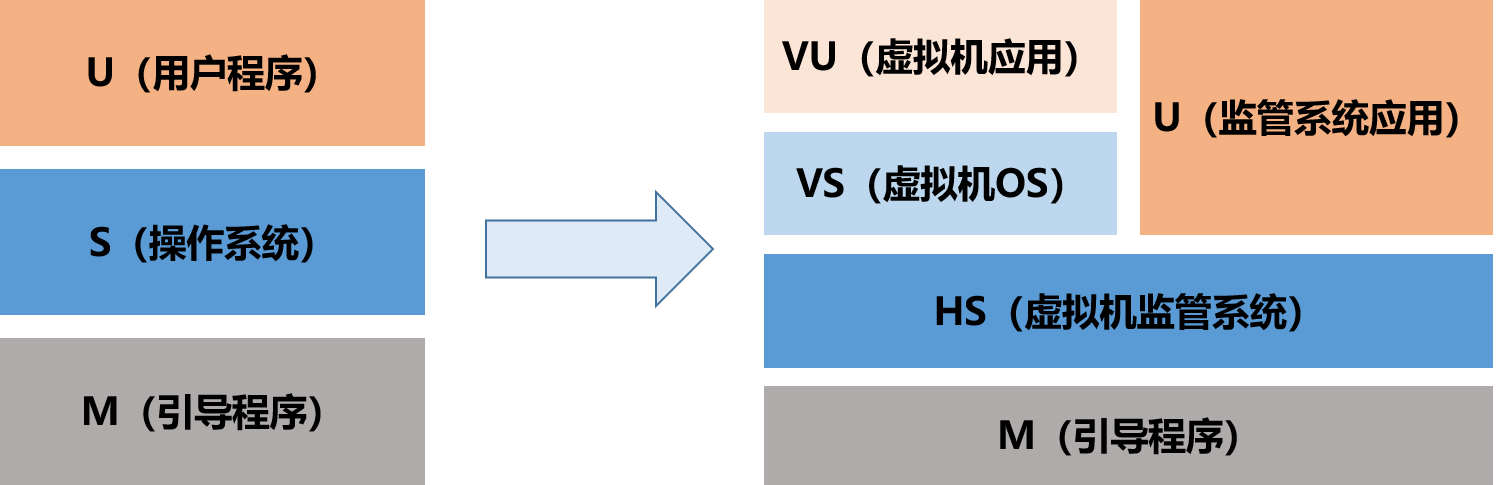
\includegraphics[scale=0.5]{priv-mode.png}
    \caption{RISC-V虚拟化扩展特权等级变化}
    \label{fig:priv-mode}
\end{figure}

控制状态寄存器(Control Status Register,CSR)是RISC-V处理器中的一组特殊寄存器,
用于控制处理器的行为和存储处理器的状态信息。
这些寄存器包含了处理器的核心控制逻辑和状态信息,可以被软件访问和操作。
虚拟化扩展下,控制管理寄存器的一个最主要的变化是添加了一套在虚拟监管模式下使用的,
用于处理虚拟机中的异常自陷的流程的寄存器,例如配置自陷地址的vstvec、保存异常指令地址的vsepc。
尽管在原始的控制状态寄存器中原本就存在用于处理监管级别的异常自陷流程的寄存器,例如stvec和sepc。
但是相同功能的寄存器重复实现一份,能够使得虚拟机中出现异常时可以自己处理,不必自陷到虚拟机管理系统中。
另一个变化是添加了一些虚拟机管理系统使用寄存器,用于配置管理系统可以捕获的虚拟机内执行的特殊指令(hstatus),
虚拟机的中断注入和委托(hedeleg、hideleg、hgeip、hgeie)等。
因此,在中断异常的种类方面,原始的监管模式下所有的中断需要在虚拟机管理模式和虚拟监管模式中各实现一次。
此外,虚拟机管理模式还需要添加一个虚拟机外部中断,用于实现虚拟机直通中断。

特权管理相关的另一部分是虚拟机管理模式下的特权指令和新增的缺页异常,
这为程序员提供管理虚拟地址翻译的方法。
未实现虚拟化扩展时,已有的SFENCE.VMA指令可被用于同步页表数据结构。
相对的,虚拟化扩展下新增了HFENCE.VVMA和HFENCE.GVMA,则是用于同步第二阶段地址翻译的页表数据结构。
同时新增了HLV.width, HLVX.HU/WU, HSV.width指令,为虚拟机管理系统提供了读取虚拟机内存的方法。

\paragraph{虚拟内存}
第二阶段地址翻译是虚拟化扩展提出的重要概念,是指在虚拟化环境中进行的地址转换过程的第二个阶段。
在传统的虚拟地址翻译机制中,虚拟地址(Virtual Address)只需要经过一次多级页表翻译
即可成为物理地址(Physical Address)访问实际的内存。
在第二段地址翻译开启时,虚拟机操作系统会对内部的虚拟地址进行一次页表翻译,
即将虚拟机虚拟地址(Guest Virtual Address,GVA)翻译成虚拟机物理地址(Guest Physical Address,GPA)。
此时处理器还需要再进行一次多级地址翻译
将虚拟机物理地址翻译成主机物理地址(Host Physical Address,HPA)才能够访问内存。
图\ref*{fig:Sv39x4}以经典的三级页表——Sv39为例,展示了两者的关系。
未开启第二阶段翻译时,例如虚拟机管理程序运行时,
最多需要访问内存三次,获取三个页表项(Page Table Entry)即可完成地址翻译。
但在开启第二阶段地址翻译后,例如在虚拟监管模式下运行虚拟机,
每次访存获取下一级页表之前,都需要再经过三级页表翻译。
换言之,为了获得虚拟机的虚地址所对应的物理地址,最多需要12次的内存访问。

\begin{figure}[htbp]
    \centering
    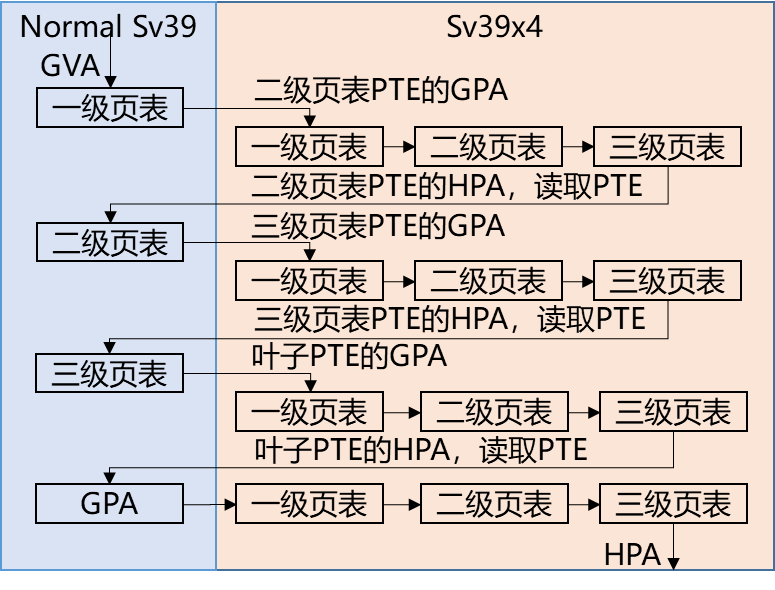
\includegraphics[scale=0.8]{Sv39x4.png}
    \caption{RISC-V虚拟化扩展的两阶段地址翻译}
    \label{fig:Sv39x4}
\end{figure}

为了管理第二阶段的地址翻译的相关信息,处理器需要提供相应的指令和控制状态寄存器用于配置。
关于控制状态寄存器,首先是第二阶段地址翻译的页目录的根地址,
保存在hgapt的寄存器中,对应于保存第一阶段地址翻译相关信息的sapt寄存器。
其次,在地址翻译的过程中不免要进行访存和权限检查,如果失败会导致处理器产生一个页错误的异常,
用于操作系统进行替换或者进一步的诊断。
因此,虚拟化扩展新增了虚拟机物理页错误的异常,对应于第二阶段地址翻译时的权限检查失败或者访存错误。
自然的,虚拟机物理页错误异常的处理程序需要触发异常的虚拟机物理地址进行诊断,
所以要求实现htval和mtval2寄存器,用于在异常触发时保存虚拟机物理地址。
可以预见,处理器的流水线内部同样需要空间保存错误地址。
特别对于取指时触发的虚拟机页错误异常,需要该指令携带地址直至执行完成退出流水线,
这对流水线中的存储部件来说是一种较大的面积开销。
对于管理虚拟内存的特权指令,在上文也有提及,包括同步指令和特权访存指令。
同步指令用于同步第二阶段页表翻译单元数据结构,包括HFENCE.VVMA和HFENCE.GVMA指令。
这两条指令的执行效果是让该指令后所有的指令执行所需的页表翻译都使用内存中最新的页表数据。
特权访存指令包括HLV.width, HLVX.HU/WU, HSV.width指令,
实际执行效果是在虚拟机管理模式下开启第二阶段地址翻译进行访存。

\section{“香山”处理器的内存管理单元}
未实现虚拟化扩展的“香山”处理器的内存管理单元的整体结构如图\ref{fig:origin-mmu}所示,可分为如下两部分:
分布式的一级页表缓存(Level 1 Translation Lookaside Buffer,L1 TLB)和
集中式的地址映射引擎(Address Mapping Enging, AME),主要包括页表翻译单元(Page Table Walker)和
二级页表缓存(Level 2 Translation Lookaside Buffer,L2 TLB)。

\begin{figure}[htbp]
    \centering
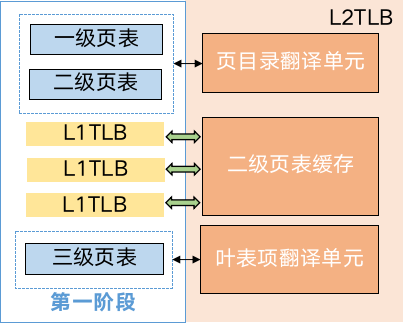
\includegraphics[scale=0.9]{origin-mmu.png}
    \caption{“香山”处理器原始内存管理单元架构}
    \label{fig:origin-mmu}
\end{figure}

\paragraph{一级页表缓存} 
一级页表缓存分布在处理器各个需要地址翻译的流水线中,例如前端的指令缓存、指令预取,后端的访存流水线。
一级页表缓存的缓存条目记录虚地址对应的多级页表翻译后的最终物理地址,因此可以实现地址翻译请求的快速的回应。
缓存条目的组织方式是全相连映射,同时每个缓存条目由使用直接映射的组织方式,存储了多个翻译结果。

\paragraph{地址映射引擎} 
当一级页表缓存不命中时,会发送翻译请求到地址映射引擎。
地址映射引擎包括一个大型的二级页表缓存、页表翻译单元以及各种权限检查模块,例如PMP和PMA。
二级页表缓存的每个条目记录了虚地址对应的各级页表,可支持各级的地址翻译请求,
具体而言,包括4KB、2MB、1GB三种大小的页表。
当翻译请求无法在页表缓存中找到,翻译请求会发送至页表翻译单元,包括页目录翻译单元和叶表项翻译单元。
页目录翻译单元负责第一级页表和第二级页表的查询,是一个朴素的阻塞自动机实现。
叶表项翻译单元负责第三级页表的查询,使用猝发传输(Burst Transfers)实现高并发。
二级页表缓存会根据请求的命中级数,将对应的翻译请求转发给对应的模块,尽可能减少实际的内存访问。
简而言之,二级页表缓存作为地址映射引擎的中心,负责一级页表缓存不命中时的三级页表翻译,
当二级页表缓存不命中时,会将请求转发给翻译单元,翻译单元通过访问内存,将翻译结果回填至二级页表缓存。

\section{处理器设计的调试及评测平台}
在传统的处理器设计流程中,常用的平台包括硬件描述语言(Hardware Description Language,HDL)建模、
逻辑分析仪(Logic Analyzer)、软件仿真工具(Simulation Tools)
和现场可编程逻辑门阵列(Field-Programmable Gate Array,FPGA)。
然而,这些方法存在一些局限性,导致开发效率较低。

在调试方面,逻辑分析仪的软件仿真可以帮助观测硬件设计在外界激励下的行为。
通过数学模型和计算机算法模拟硬件设计,获取设计中各个信号值随时间的变化曲线,即波形图。
尽管波形图和仿真软件可以帮助工程师了解电路内部的所有状态,是错误调试的基础,
但是当需要在各种复杂场景下进行调试时,仍旧存在许多缺陷。
第一,波形重放在发现错误信号的能力有限。
单一信号的微小错误会被淹没在巨大的细节中,很可能数千万个周期后才会暴露。
因此,学术界近年来提出了使用架构模拟器和差分测试的方法。
通过比对正确的体系结构信息,精确定位出错现场。
第二,仿真工具执行速度远低于FPGA,这是由于可并行性低、同步要求高等自身特性决定的。
尽管在开源社区和学术界存在许多高效的解决方案,
例如iverilog\cite{github:iverilog}、
verilator\cite{github:verilator}和manticore\cite{asplso23manticore}。
但在运行大型基准测试和系统软件时,花费的时间仍然不可接受。
这个缺陷仍然没有可解决的方案,时至今日也是学术界研究的热点。

在评测方面,FPGA被广泛运用于原型验证。
通过将处理器设计部署在物理的逻辑门和寄存器中,
FPGA能够提供更真实的测试环境和远快于软件仿真的运行速度。
同时,在FPGA中实现特定硬件的时间开销远小于通过流片方式生产的开销。
但是,FPGA由于其硬件特性,能够获取的波形信号和时间范围十分受限。
只能通过对外部设备的输出,判断硬件设计是否存在错误,无法提供调试所需的电路内部信息。
基于上述缺陷,学术界提出了一种通过FPGA加速软件仿真的方案——REMU\cite{iccd2023remu},
通过将FPGA某一运行时刻的所有寄存器和存储器信息,精确重放到仿真软件中。
利用仿真软件生成波形的能力来帮助调试。
本文中也使用了该方法发现硬件设计的错误,提高了开发效率。

\section{研究方案}

今天,云数据中心服务提供商在迅速地发展,市场中可见的各种云服务,其根本的底层技术都是处理器虚拟化。
在市场需求的刺激下,处理器芯片的主流架构,例如Intel和ARM都提供了虚拟化的硬件支持。
近年来,RISC-V作为一个新兴的开放指令集,也开始着手云数据中心的需求。
然而,如上文虚拟化扩展的软硬件支持所述,关于RISC-V处理器的虚拟化技术的研究还十分有限,
特别是高性能处理器在虚拟化扩展方面的相关研究。
尽管Rocket Chip和CVA6实现了虚拟化扩展,但他们都是单发射处理器。
因此,高性能RISC-V处理器的虚拟化扩展相关的研究亟待进行。
本文尝试填补这一空缺,研究内容包括处理器硬件扩展到虚拟化软件,以及全系统的虚拟化性能评估。

硬件方面,本文着手“香山”项目——目前国际上性能最高的RISC-V处理器核。
尝试在“香山”中实现虚拟化扩展,主要包括特级管理单元、内存管理单元的扩展。
特别是内存管理单元,本文尝试了各种能够加快速度、提高吞吐量的微架构。
相比Rocket Chip的最朴素的实现,“香山”实现了支持VMID和ASID的虚拟内存屏障指令,
这能够减少屏障指令执行时无效化的缓存条目,加快地址翻译的速度。
CVA6实现了第二阶段专用的页表缓存,被称为GTLB,并表明该微架构能够加速第二阶段页表翻译单元的速度。
“香山”的微架构设计与其和而不同,通过在二级页表缓存存放两阶段的页表,
同时在进行第二阶段页表翻译前查询二级页表缓存。
该方案实现了类似的第二阶段专用是页表缓存的效果,而且最小化对原有设计的修改,没有额外的缓存面积开销。
尽管CVA6和Rocket Chip均实现了二级页表缓存,但“香山”是首个将二级页表缓存用于第二阶段页表的开源RISC-V处理器。
除此之外,“香山”在一级页表缓存以及页表翻译单元均有其他能够提高吞吐、加快速度的微架构设计。
这些设计对虚拟化性能能够产生何种效果,同样具有巨大的研究价值,能够为后来者提供了设计思路和经验。

虚拟化软件方面,本文尝试适配Linux-KVM——经典的Type2虚拟机管理系统。
尽管KVM在软件方面的适配工作已经实现,在RISC-V处理器模拟器中也可以运行。
但是在开源RISC-V处理器硬件中,尚未有成熟的KVM解决方案,包括Rocket Chip和CVA6。
而且,KVM在云服务数据中心中被广泛应用,因此以KVM作为软件适配的目标十分必要。
作为Type2虚拟机管理系统,使用KVM启动虚拟机的前提是启动Linux主机系统,
因此本文先使用虚拟化扩展后的“香山”启动了Linux,并在主机系统中进行了性能测试作为基准线。
之后,尝试在命令行中通过kvmtool启动虚拟机,但是由于硬件中潜在的问题导致KVM启动失败。
为了调试的硬件错误,本文尝试了多种现有的常规调试工具:
基于逻辑仿真软件的差分测试、基于FPGA的加速仿真平台。
但是现有的调试工具能力有限,在复杂的软硬件联合调试中难以解决问题。
特别是在本文中尝试启动虚拟机的场景下,逻辑仿真软件的运行速度十分缓慢,
基于FPGA的加速仿真平台也无法精确定位错误现场。
为解决硬件潜在的错误,急需一个能够快速定位错误现场且能够解析硬件体系结构信息的调试工具。
这对于本文,甚至是处理器设计验证的学术研究领域中,都是极具有价值的课题方向。
因此,本文也基于现有的调试工具进行了一些改进和探索。

\section{本章小结}
本章首先介绍RISC-V虚拟化扩展,特别是虚拟内存部分提出的第二阶段地址翻译,
是本文硬件设计方案一个需要着重处理的部分。
第二,介绍“香山”处理器的内存管理单元的原始架构,因为本文的总体设计方案基于“香山”南湖架构。
在第三章会直接介绍虚拟化扩展下的内存管理单元,此处对原始架构的说明能够帮助理解。
第三,介绍本文所使用的所有调试工具和评测平台,能够帮助后文实验部分的理解。
最后,会结合RISC-V虚拟化扩展软硬件的相关工作,对比着介绍本文的整体研究方案。